%
% $RCSfile: human_thinking.tex,v $
%
% Copyright (C) 2002-2008. Christian Heller.
%
% Permission is granted to copy, distribute and/or modify this document
% under the terms of the GNU Free Documentation License, Version 1.1 or
% any later version published by the Free Software Foundation; with no
% Invariant Sections, with no Front-Cover Texts and with no Back-Cover
% Texts. A copy of the license is included in the section entitled
% "GNU Free Documentation License".
%
% http://www.cybop.net
% - Cybernetics Oriented Programming -
%
% http://www.resmedicinae.org
% - Information in Medicine -
%
% Version: $Revision: 1.1 $ $Date: 2008-08-19 20:41:07 $ $Author: christian $
% Authors: Christian Heller <christian.heller@tuxtax.de>
%

\section{Human Thinking}
\label{human_thinking_heading}
\index{Human Thinking}

Knowledge as created by the human mind is learned by associating information,
by embedding it in a \emph{Context}, as investigated by \emph{Pragmatics}, a
subfield of linguistics \cite{wikipedia}. It is thus built of structured,
inter-related data (definitions given in section
\ref{knowledge_engineering_heading}). The interesting question explored in this
section is what kind of structures and relations are used in knowledge models
as known from nature, that is \emph{Human Thinking}?

%
% $RCSfile: basic_behaviour.tex,v $
%
% Copyright (C) 2002-2008. Christian Heller.
%
% Permission is granted to copy, distribute and/or modify this document
% under the terms of the GNU Free Documentation License, Version 1.1 or
% any later version published by the Free Software Foundation; with no
% Invariant Sections, with no Front-Cover Texts and with no Back-Cover
% Texts. A copy of the license is included in the section entitled
% "GNU Free Documentation License".
%
% http://www.cybop.net
% - Cybernetics Oriented Programming -
%
% http://www.resmedicinae.org
% - Information in Medicine -
%
% Version: $Revision: 1.1 $ $Date: 2008-08-19 20:41:05 $ $Author: christian $
% Authors: Christian Heller <christian.heller@tuxtax.de>
%

\subsection{Basic Behaviour}
\label{basic_behaviour_heading}
\index{Basic Behaviour in Nature}
\index{A new Kind of Science}
\index{Repetition}
\index{Nesting}
\index{Randomness}
\index{Localised Structures}
\index{Principle of Universality}

Starting from a neutral view to understanding the universe -- and science in
general -- Stephen Wolfram studied the abstract world of rules put into simple
computer programs. \textit{He took the lessons from what kinds of things occur
there and had them in mind when investigating natural systems}, as
\cite{wikipedia} writes. Wolfram's book \emph{A new Kind of Science}
\cite{wolfram} argues that the universe is made up of four basic types of
behaviour (figure \ref{behaviour_figure}):

\begin{enumerate}
    \item \emph{Repetition}
    \item \emph{Nesting}
    \item \emph{Randomness}
    \item \emph{Localised Structures}
\end{enumerate}

\begin{figure}[ht]
    \begin{center}
        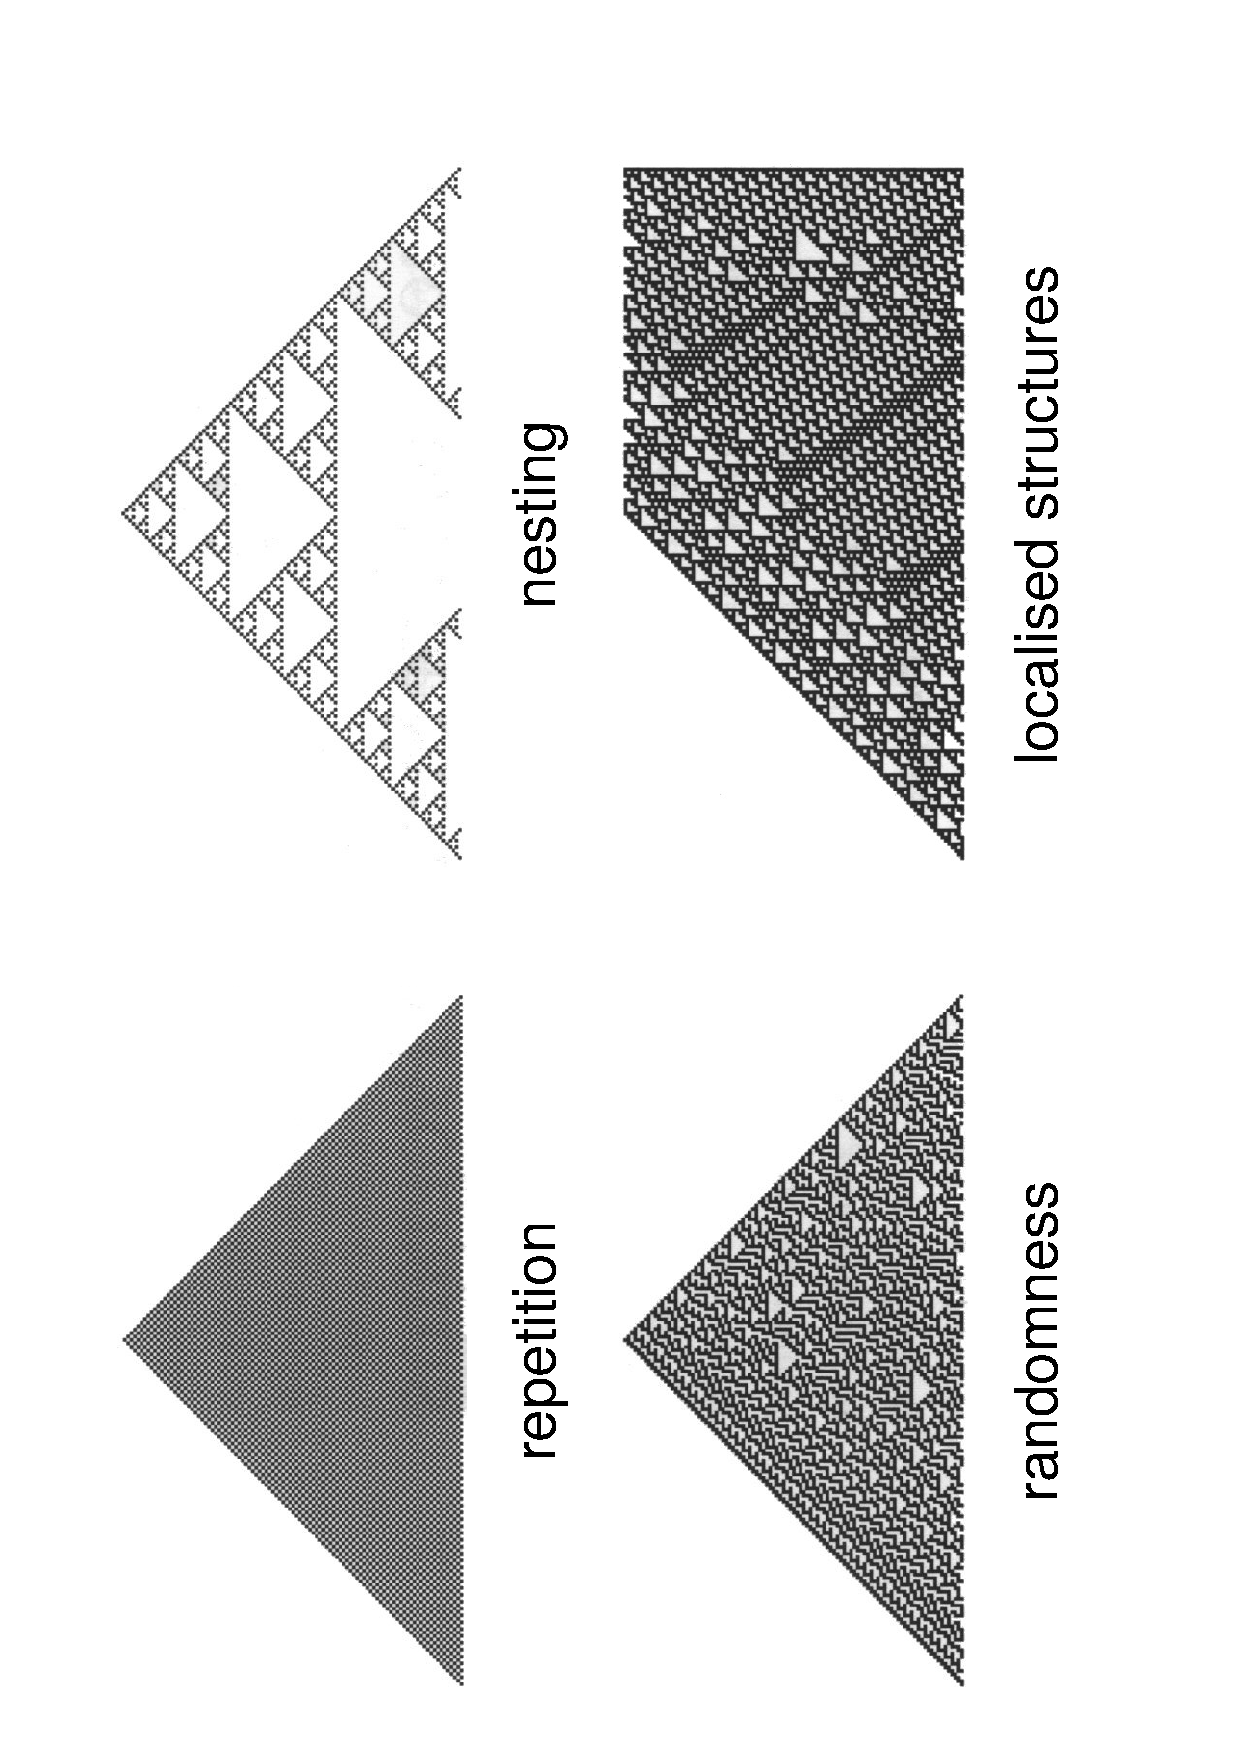
\includegraphics[scale=0.3,angle=-90]{graphic/behaviour.pdf}
        \caption{Wolfram's Four Basic Kinds of Behaviour \cite{wolfram}}
        \label{behaviour_figure}
    \end{center}
\end{figure}

These types of behaviour, after Wolfram, were present everywhere, in nature as
in the whole universe. Just everything in existence contained at least one of
these structures and all sciences were affected by them. Yet while Wolfram
applies results of computing to the study of nature, this work follows the exact
opposite way in that it observes phenomenons of nature and concepts used in
other sciences, and tries to apply them to the design of software systems.
Without knowing a final answer -- the unexpected surprise is that at least two
of Wolfram's findings of basic behaviour match to abstractions as known from
human thinking, and have a pendant in this work:

\newpage

\begin{enumerate}
    \item \emph{Repetition} is the recurrence of equal structures. Yet before
        structures can be compared, they have to be demarcated. This is what
        section \ref{abstraction_heading} will call \emph{Discrimination}
        (later \emph{Itemisation}), and also \emph{Categorisation}.
    \item \emph{Nesting} creates the famous, beautiful \emph{Fractals}. It is
        somewhat similar to \emph{Repetition}, only that the repeated
        structures are not equal in size and do not occur along some chain.
        While the infinity of \emph{Repetition} lies in its neverending
        \emph{Continuation} along some line(s) on the same level, it lies in
        the \emph{Diving} into a deeper level for \emph{Nesting}. Section
        \ref{abstraction_heading} will call this \emph{Composition}.
\end{enumerate}

Wolfram defines a \emph{Principle of Universality} which states that in fact
\emph{all} kinds of systems, even very simple ones, are capable of showing
complex behaviour in form of \emph{Localised Structures}, once some threshold
in the complexity of the underlying rules is passed. But where is this threshold
and who defines what complex behaviour actually is? Does a threshold exist at
all or are the four kinds of behaviour in fact not different? Indeed, one could
argue that neither \emph{Repetition}, nor \emph{Nesting}, nor \emph{Randomness}
are anything special and that it is just the human mind interpreting them as
something special, as assumed by this work. It claims that the human mind gives
structure and meaning to the surrounding real world by building a virtual world.
The principles of human thinking are therefore investigated in the next sections.

Software abstracts human thought which, in order to understand and act in the
surrounding real world, needs to recognise and rely on \emph{known} patterns.
\emph{Randomness} and \emph{Localised Structures} in Wolfram's meaning,
although existent in universe, are rather not used by the human mind to store
information, nor do they seem useful for the design of deterministic software
systems. Of course, information can arrive at- and influence a human mind in an
arbitrary manner and be associated randomly, at will. But the concepts it forms
need to be stable in order to build up knowledge. The research done in this
work therefore relies on reproducible structures making sense to human minds,
namely \emph{Repetition} and \emph{Nesting}.

%
% $RCSfile: conglomerate.tex,v $
%
% Copyright (C) 2002-2008. Christian Heller.
%
% Permission is granted to copy, distribute and/or modify this document
% under the terms of the GNU Free Documentation License, Version 1.1 or
% any later version published by the Free Software Foundation; with no
% Invariant Sections, with no Front-Cover Texts and with no Back-Cover
% Texts. A copy of the license is included in the section entitled
% "GNU Free Documentation License".
%
% http://www.cybop.net
% - Cybernetics Oriented Programming -
%
% http://www.resmedicinae.org
% - Information in Medicine -
%
% Version: $Revision: 1.1 $ $Date: 2008-08-19 20:41:06 $ $Author: christian $
% Authors: Christian Heller <christian.heller@tuxtax.de>
%

\subsection{Conglomerate}
\label{conglomerate_heading}
\index{Universe as Conglomerate}

\emph{Universe} is the most general word describing everything humans think
exists. Whether it exists in reality or just as an illusion in their minds, is
a fundamental question of philosophy and will not be discussed here. The author
of this document assumes that a \emph{Real World} exists and humans only
\emph{reflect} but not \emph{construct} it in their minds.

\begin{figure}[ht]
    \begin{center}
        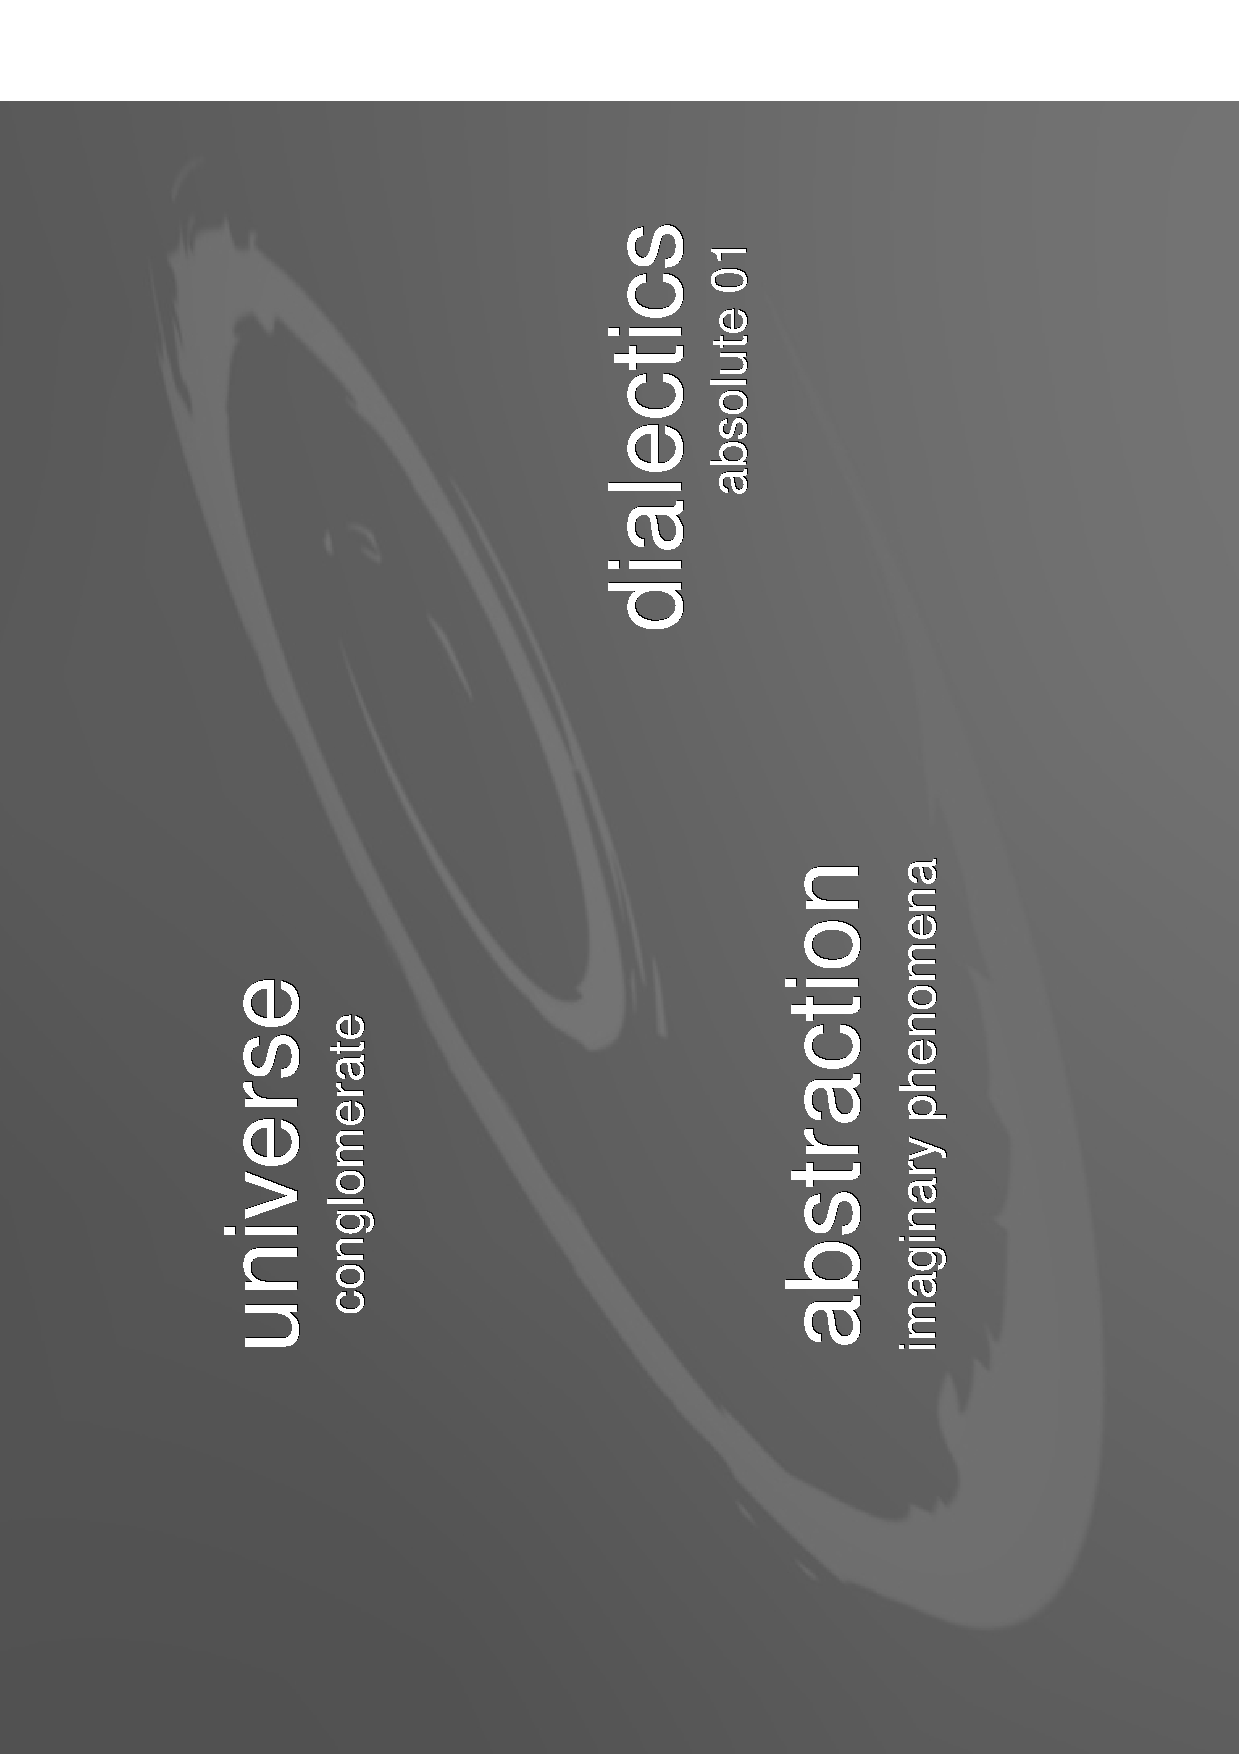
\includegraphics[scale=0.3,angle=-90]{graphic/conglomerate.pdf}
        \caption{The Universe as to-be-abstracted Conglomerate (swirl from \cite{debian})}
        \label{conglomerate_figure}
    \end{center}
\end{figure}

The whole universe can be seen as \emph{Conglomerate} of everything in
existence (figure \ref{conglomerate_figure}). Computer systems enable humans to
abstract things to just two states labelled \emph{0} and \emph{1} (section
\ref{hardware_architecture_heading}), on a very low level. Human systems use
more high-level methods for abstraction. Common concepts to describe a
real-world environment are \emph{Particle}, \emph{Dimension} or \emph{Force}.
Everybody will know more of them. But what is a particle?

%
% $RCSfile: abstraction.tex,v $
%
% Copyright (C) 2002-2008. Christian Heller.
%
% Permission is granted to copy, distribute and/or modify this document
% under the terms of the GNU Free Documentation License, Version 1.1 or
% any later version published by the Free Software Foundation; with no
% Invariant Sections, with no Front-Cover Texts and with no Back-Cover
% Texts. A copy of the license is included in the section entitled
% "GNU Free Documentation License".
%
% http://www.cybop.net
% - Cybernetics Oriented Programming -
%
% http://www.resmedicinae.org
% - Information in Medicine -
%
% Version: $Revision: 1.1 $ $Date: 2008-08-19 20:41:05 $ $Author: christian $
% Authors: Christian Heller <christian.heller@tuxtax.de>
%

\subsection{Abstraction}
\label{abstraction_heading}
\index{Abstractions of Human Thinking}
\index{Item}
\index{Category}
\index{Compound}

Humans understand their environment by building simplified models (concepts) of
it. These are based on fundamental \emph{Abstractions} like \emph{Item},
\emph{Category} or \emph{Compound} (figure \ref{abstraction_figure}), which are
the topic of this section. Part of it was already published in \cite{heller2004}.

\begin{figure}[ht]
    \begin{center}
        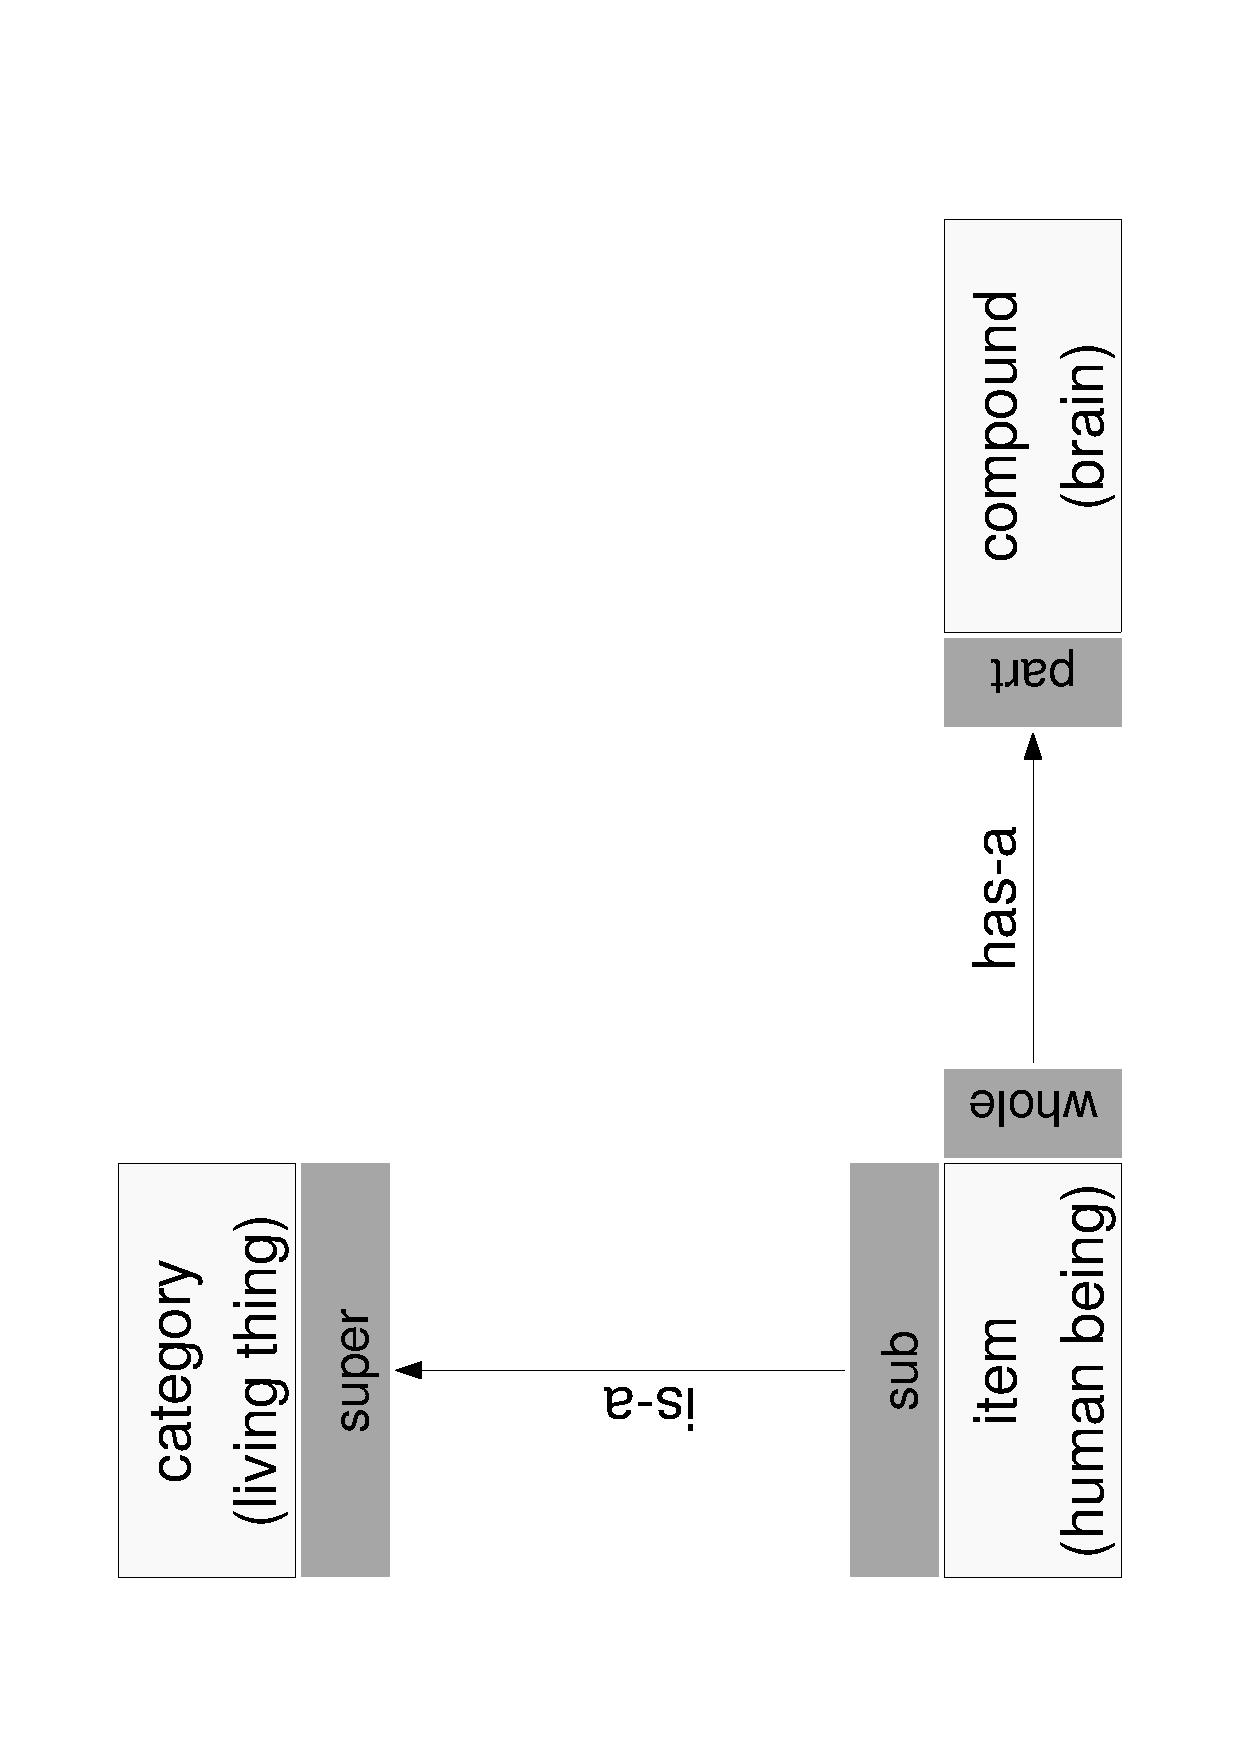
\includegraphics[scale=0.3,angle=-90]{graphic/abstraction.pdf}
        \caption{Abstractions of Human Thinking}
        \label{abstraction_figure}
    \end{center}
\end{figure}

%
% $RCSfile: item.tex,v $
%
% Copyright (c) 2001-2004. Christian Heller. All rights reserved.
%
% No copying, altering, distribution or any other actions concerning this
% document, except after explicit permission by the author!
% At some later point in time, this document is planned to be put under
% the GNU FDL license. For now, _everything_ is _restricted_ by the author.
%
% http://www.cybop.net
% - Cybernetics Oriented Programming -
%
% http://www.resmedicinae.org
% - Information in Medicine -
%
% @author Christian Heller <christian.heller@tuxtax.de>
%

\subsection{Item}
\label{item_heading}

As first and most important abstraction, the human brain divides its real-world
environment into discrete \emph{Items}. Physicists call smaller items \emph{Particle}.
Plenty of other synonyms exist. Software developers often talk of \emph{Object}.
This document preferrably uses the more neutral name \emph{Item}, since models
are created not only of objects but also of \emph{Subjects}.

Behavioural psychologists talk of this ability as \emph{Discrimination}. It commonly
focuses on a specific real world phenomenon, leaving out parameters which are not
interesting in the given context. This is necessary because otherwise, a brain
would have to model and capture the whole universe (with every single particle
being duplicated), which is obviously impossible. As example, a \emph{Human Being}
as item is stated (in parentheses) in figure \ref{human_thinking_figure}.

Not only human beings, but also some higher animal species (like apes) are able
to \emph{discriminate} their environment and to form terms to name it.
Additionally, they have a primitive \emph{Self Concept}, that is a term for
their own personality. However, their cognitive abilities are limited in that
concepts are only available in the presence of the corresponding item. Jaeger
\cite{jaeger} calls that \emph{Online Thinking}; cognition scientists speak of
\emph{Terms of first Order} or \emph{Sensoric Type of Terms}.

Contrary to this, the more advanced \emph{Offline Thinking} allows humans to
think about items they currently cannot sense. Cognition scientists here speak of
\emph{Terms of second Order}. They became possible by \emph{associating} sensoric
signals with terms of a language. The resulting \emph{Net of Associations} brought
a number of advantages \cite{jaeger}:

\begin{itemize}
    \item{\emph{Decoupling} thinking from immediate motoric reaction}
    \item{\emph{Time Index} in scenes so that past memories can be\\
        recalled, the future be planned}
    \item{\emph{Dual Representation} of online and offline contents}
    \item{\emph{Self Awareness} thanks to online and offline thinking}
    \item{\emph{Associations} increasing the expressiveness of terms}
\end{itemize}

%
% $RCSfile: category.tex,v $
%
% Copyright (C) 2002-2008. Christian Heller.
%
% Permission is granted to copy, distribute and/or modify this document
% under the terms of the GNU Free Documentation License, Version 1.1 or
% any later version published by the Free Software Foundation; with no
% Invariant Sections, with no Front-Cover Texts and with no Back-Cover
% Texts. A copy of the license is included in the section entitled
% "GNU Free Documentation License".
%
% http://www.cybop.net
% - Cybernetics Oriented Programming -
%
% http://www.resmedicinae.org
% - Information in Medicine -
%
% Version: $Revision: 1.1 $ $Date: 2008-08-19 20:41:05 $ $Author: christian $
% Authors: Christian Heller <christian.heller@tuxtax.de>
%

\subsubsection{Category}
\label{category_heading}
\index{Category}
\index{Offline Thinking}
\index{Terms of Second Order}
\index{Categorisation}
\index{Type}
\index{Class}
\index{Common Characteristics}
\index{Systematics of Nature}
\index{Classification}
\index{Systematics}
\index{Generalisation}
\index{Specialisation}
\index{Is-a Relationship}
\index{Super Category}
\index{Sub Category}
\index{Parent Category}
\index{Child Category}
\index{Object Oriented Programming}
\index{OOP}
\index{Inheritance}

Offline thinking (in terms of second order) enables humans not only to
discriminate items but also to \emph{categorise} them into superior groups.
Since it is impossible to exactly model the real world in complete, compromises
have to be made: People do not model every single item in their minds but rather
group them into \emph{Types} (\emph{Classes}) of common characteristics.

\begin{figure}[ht]
    \begin{center}
        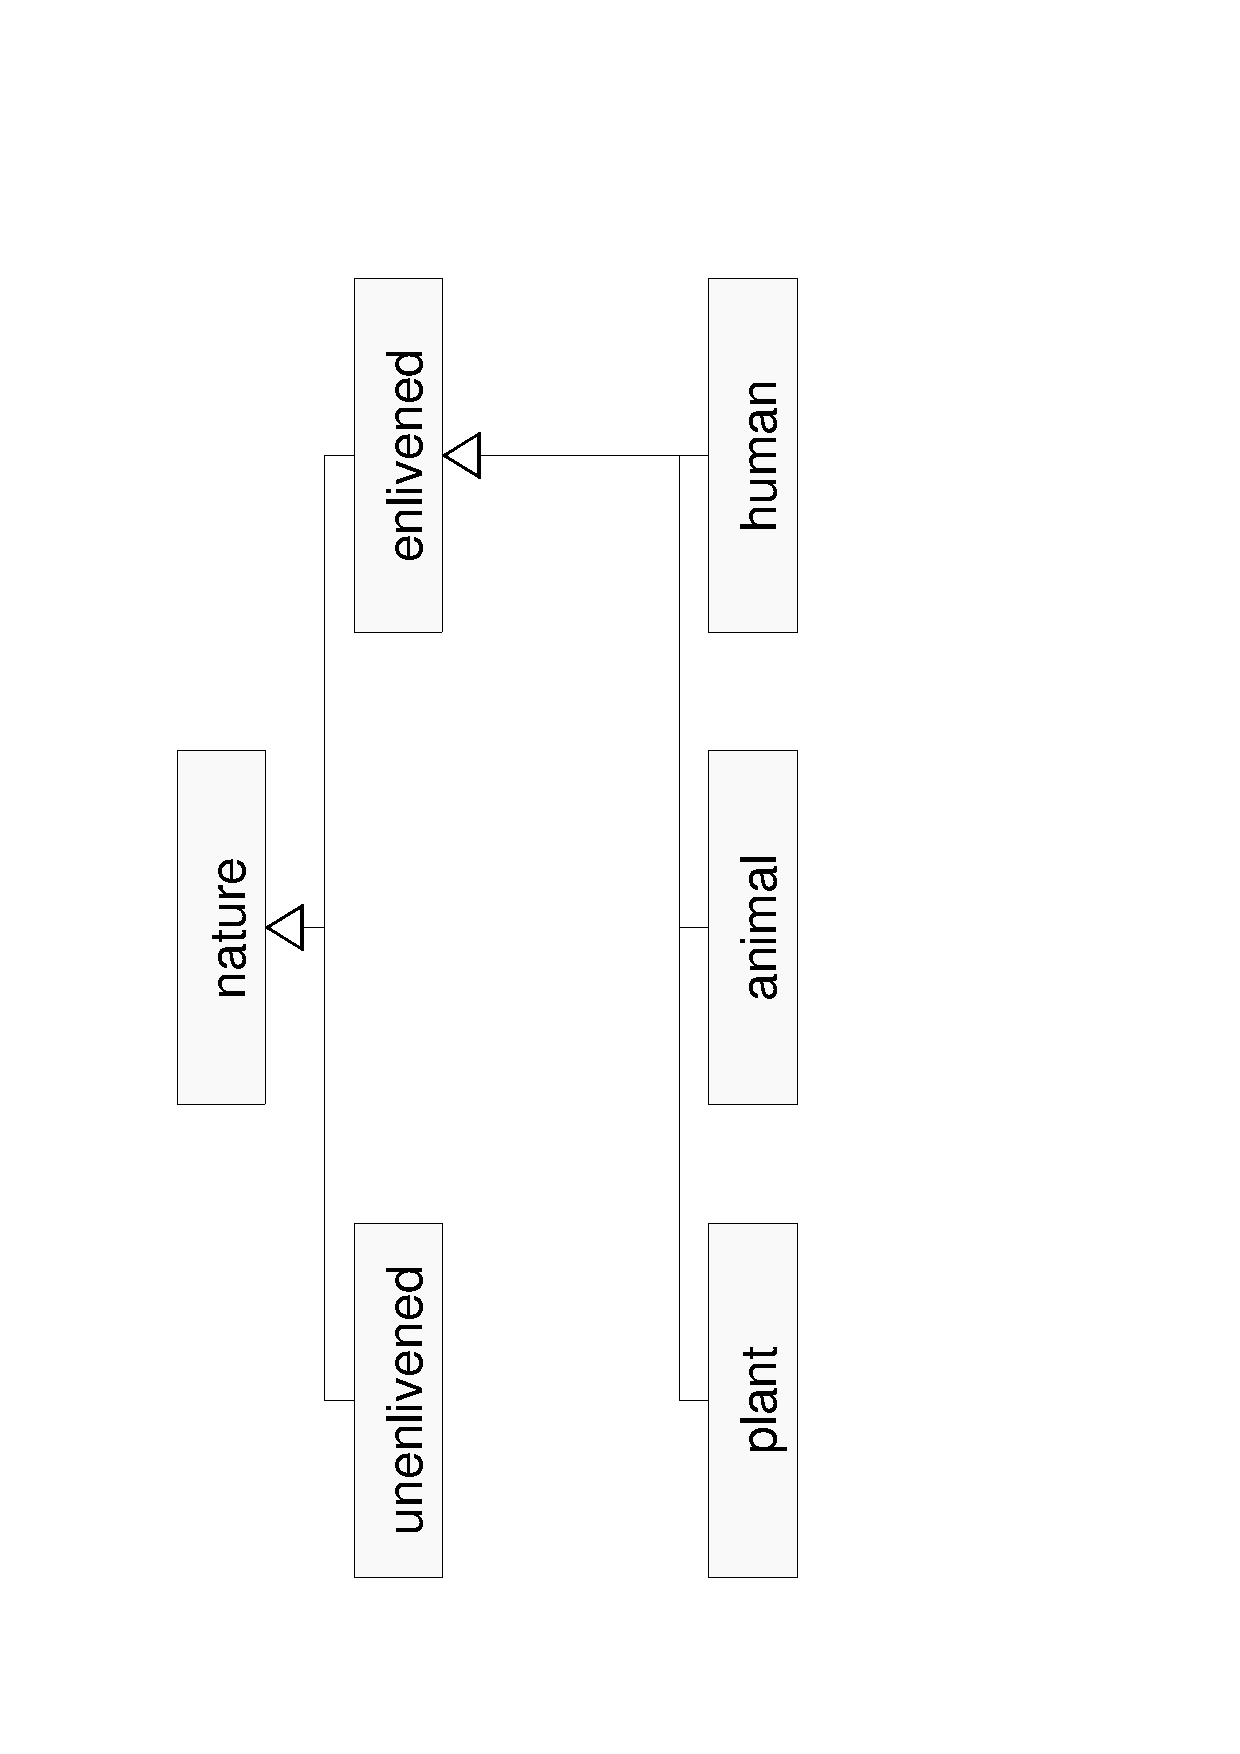
\includegraphics[scale=0.3,angle=-90]{graphic/nature.pdf}
        \caption{Systematics of Nature}
        \label{nature_figure}
    \end{center}
\end{figure}

This kind of classification stems from the earliest days of ancient science.
\emph{Plato}'s (429-347 B.C.) pupil \emph{Aristotle} (384-322 B.C.), being the
teacher of \emph{Alexander the Great}, was the first philosopher who logically
captured and organised the world. It was him who sorted items into clear groups
which he called \emph{Categories}. And it was him who first distinguished
between \emph{enlivened} and \emph{unenlivened} nature; who parted living forms
into \emph{Plants}, \emph{Animals} and \emph{Humans}. The science of biology
calls this classification a \emph{Systematics} (figure \ref{nature_figure}).

\emph{Categorisation} (classification) can be seen from two sides, depending on
what direction of that relationship one wants to emphasise. Taking Aristotle's
examples, \emph{Living Thing} would be a \emph{Generalisation} of \emph{Plants},
\emph{Animals} and \emph{Humans}. \emph{Animal} would be a \emph{Specialisation}
of \emph{Living Thing}.

Software developers often call categorisation an \emph{is-a} relationship and
talk of \emph{Super} and \emph{Sub} categories (sometimes also \emph{Parent}
and \emph{Child} categories). Section \ref{inheritance_heading} described how
\emph{Object Oriented Programming} (OOP) uses categorisation to let a sub class
inherit attributes and methods from its super class.

%
% $RCSfile: compound.tex,v $
%
% Copyright (c) 2001-2004. Christian Heller. All rights reserved.
%
% No copying, altering, distribution or any other actions concerning this
% document, except after explicit permission by the author!
% At some later point in time, this document is planned to be put under
% the GNU FDL license. For now, _everything_ is _restricted_ by the author.
%
% http://www.cybop.net
% - Cybernetics Oriented Programming -
%
% http://www.resmedicinae.org
% - Information in Medicine -
%
% @author Christian Heller <christian.heller@tuxtax.de>
%

\subsection{Compound}
\label{compound_heading}

\emph{Composition} is the third kind of abstraction that humans use to understand
their environment. It is an important instrument for the human mind to associate
information, that is to acquire, store and recall \emph{Knowledge}. Every item is
recognized as a \emph{Compound} of smaller items and can therefore also be called
\emph{Tree} or \emph{Hierarchy}. The subject of \emph{Artificial Intelligence} (AI)/
\emph{Knowledge Engineering} talks of \emph{Concept} or \emph{Schema}.

In software design, the terms \emph{Parent} and \emph{Child} are often used to
describe both, the items in a composition as well as the items in a categorization
relationship (section \ref{category_heading}).
To avoid misunderstandings, this document sticks to the terms \emph{Super} and
\emph{Sub} for categorization and to the terms \emph{Whole} and \emph{Part}
\cite{sowa} for composition. Yet other terms to describe items of a composition
would be \emph{Container} and \emph{Element}.

To stick with the example of a \emph{Human Being}, one could say that it is
composed of \emph{Organs} such as \emph{Eye}, \emph{Ear}, \emph{Heart},
\emph{Brain}, \emph{Arm} and further, also smaller parts. Other examples are the
concept of an \emph{Atom} consisting of a \emph{Core} and \emph{Electrons} or
that of a physical \emph{Book} composed of a \emph{Paperback Cover} and
\emph{Paper Pages}.
However, knowledge representation always depends on what one wants to express in
which context. The \emph{Book}, for example, can be represented in many other
ways. Logically, it is usually separated into \emph{Part}, \emph{Chapter},
\emph{Section}, \emph{Paragraph}, \emph{Sentence}, \emph{Word} and \emph{Character}.

It is important to note the \emph{unidirectional} kind of relations: A human
being is composed of organs but an organ is never composed of a human being!

Not only \emph{static} items represent a compound; \emph{dynamic} items are
hierarchical as well. The process \emph{Take Book from Library}, for example,
may have the following structure:

\begin{itemize}
    \item{Check Catalogue}
    \begin{itemize}
        \item{Investigate suitable Books}
        \item{Note Registration Number}
    \end{itemize}
    \item{Organize Book}
    \begin{itemize}
        \item{Look for Shelf}
        \item{Take off Book}
    \end{itemize}
    \item{Borrow Book}
\end{itemize}

Returning to human thinking, one realizes that in the end, everything in universe
can be put into variable hierarchical models, that is consists of smaller items
and belongs to a bigger item. From the physical point of view, nobody knows where
this hierarchy really stops, towards \emph{Microcosm} as well as towards
\emph{Macrocosm}. There is no \emph{absolute}, \emph{basic} item.
A \emph{Particle} as concept exists only in the human mind, placed somewhere
between micro- and macrocosm, with hypothetic borders.


%
% $RCSfile: interaction.tex,v $
%
% Copyright (c) 2001-2004. Christian Heller. All rights reserved.
%
% No copying, altering, distribution or any other actions concerning this
% document, except after explicit permission by the author!
% At some later point in time, this document is planned to be put under
% the GNU FDL license. For now, _everything_ is _restricted_ by the author.
%
% http://www.cybop.net
% - Cybernetics Oriented Programming -
%
% http://www.resmedicinae.org
% - Information in Medicine -
%
% @author Christian Heller <christian.heller@tuxtax.de>
%

\subsection{Interaction}
\label{interaction_heading}

As explained in previous sections, every abstract model is a \emph{Compound} of
smaller \emph{Parts}. What does this relation imply? What does a compound
\emph{know} about its parts? Knowledge \emph{about} something is often called
\emph{Meta Information}.

The most obvious way to uniquely identify parts is to give them a \emph{Name}. The
concept of a human body, for example, has parts like \emph{Heart}, \emph{Left Arm}
or \emph{Skin}. Secondly, a compound needs to know about the \emph{Model} of each
part which may be a compound itself. But what about other knowledge like
the order or position of parts within their compound?

To find an answer, the science of \emph{Psychology} needs to be called in. It
distinguishes between various aspects of a (visual) impression of the human mind,
as there are \emph{Shape}, \emph{Depth}, \emph{Color} or \emph{Movement}
\cite{stoerig}. Looking closer at these, one realizes that they are representations
of the classical physical dimensions that humans use to describe the world:

\begin{itemize}
    \item{\emph{Movement}: changing the state of something over \emph{Time}}
    \item{\emph{Shape}: how items would appear in a two-dimensional world, as
        known from \emph{Geometry}}
    \item{\emph{Depth} (stereo vision): adding a third dimension to shapes, so
        that these become three-dimensional and form a \emph{Space}}
    \item{\emph{Color}: not being considered a dimension, telling about how items
        reflect \emph{Light}}
    \item{\emph{Mass}: another physical value describing the world which is not
        considered to be a dimension}
\end{itemize}

If, according to modern physics, not all of the impressions listed above are
dimensions, what is common to them? -- All can be used to express a special aspect
of a composition relation which this paper calls \emph{Composition Interaction}.

To the concept of an \emph{Atom} belong a \emph{Core} and \emph{Electrons}. The
atom provides the \emph{Space} that the core and electrons can fill with their
extension. For core and electrons, the atom represents the small universe they live
in. Moreover, the atom \emph{knows} about the \emph{Position} (\emph{Trajectory})
of each electron. Thus, one can say that the atom as a \emph{Whole} interacts with
its \emph{Parts} by means of space. Electrons, on the other hand, know nothing
about their own position within the atom; they do not know about the existence of
the atom at all. But having a size, they indirectly exert influence on the whole
atom by contributing to its overall extension in space.

A \emph{Solar System}, as concept, has very much in common with the atom. It has a
star, the \emph{Sun}, as its core and it has \emph{Planets} orbiting around that
star. Besides the composition interaction over space that also exists here, there
is another relation worth paying attention to: \emph{Mass}. Conceptually, the
solar system can be treated as a closed field of \emph{Mass}, the sun representing
the center of that mass, the planets additions. The solar system as a \emph{Whole}
knows about the masses of its \emph{Parts}, what can be considered a conceptual
interaction.

A third relation that humans use to place themselves and the environment into their
very own model of the universe is \emph{Time}. Any \emph{Process} can be split into
\emph{Sub Processes} and such represents a structure with \emph{hierarchical}
character. In most cases, the \emph{Order} in which sub processes are executed, is
very important. Without it, no meaningful \emph{Algorithm} could ever be created.
A process knows about the \emph{Occurrence} of its sub processes and this sequence
information is stored in units of time. Moreover, the \emph{Whole} process sets a
time frame that all \emph{Part} processes, in sum, cannot exceed. Their \emph{Duration}
is limited. Again, process and sub processes have some kind of composition relation;
in this case over time.

Conceptual interactions like \emph{Space}, \emph{Mass} or \emph{Time} are used by a
model to position parts within its area of validity. Yet this meta knowledge is not
enough. Frequently, parts have to be \emph{constrained} to maintain the validity of
the whole model. The concept of a \emph{Table} consists of a \emph{Top} and one to
four \emph{Legs}. The additional information herein is the \emph{Constraint} of the
number of legs to at least \emph{one} and at most \emph{four}.

Finally, what makes up the \emph{Character} of an item (in the understanding of the
human mind) is the \emph{Parts} it consists of, combined with \emph{Meta Information}
about these parts. Most properties of a molecule in \emph{Chemistry} are determined
by the number and arrangement of its atoms. \emph{Hydrogen} (H$_{2}$) becomes
\emph{Water} (H$_{2}$O) (with a totally different character) when one \emph{Oxygen}
(O) atom is added per hydrogen molecule.

Properties are based on impressions of the human mind which are often identical to
what is called a \emph{Dimension} in physics. Item \emph{Properties} that do not
result from its composed nature have to be defined additionally as size in space
(expansion), in time (duration, instant), in mass (massiness) or color as
speciality. While such dimension properties of an item are given as the
\emph{Difference} (size) of something, a conceptual interaction between a compound
and its parts is stated as \emph{Point} (position).

%
% $RCSfile: intrinsic_or_extrinsic_properties.tex,v $
%
% Copyright (C) 2002-2008. Christian Heller.
%
% Permission is granted to copy, distribute and/or modify this document
% under the terms of the GNU Free Documentation License, Version 1.1 or
% any later version published by the Free Software Foundation; with no
% Invariant Sections, with no Front-Cover Texts and with no Back-Cover
% Texts. A copy of the license is included in the section entitled
% "GNU Free Documentation License".
%
% http://www.cybop.net
% - Cybernetics Oriented Programming -
%
% http://www.resmedicinae.org
% - Information in Medicine -
%
% Version: $Revision: 1.1 $ $Date: 2008-08-19 20:41:07 $ $Author: christian $
% Authors: Christian Heller <christian.heller@tuxtax.de>
%

\subsection{Intrinsic or Extrinsic Properties}
\label{intrinsic_or_extrinsic_properties_heading}
\index{Intrinsic Property}
\index{Extrinsic Property}
\index{Position as Point}
\index{Size as Difference}
\index{Benediktine Approach}
\index{Spatial Dimension}

Properties may not only represent the \emph{Position} of a part in space/ mass/
time, but also its \emph{Size} in the same dimensions. For space, it may be
called \emph{Expansion}, for mass \emph{Massiness}, and for time \emph{Duration}.
While a size is always represented by the \emph{Difference} of two values, a
position is represented by a \emph{Point}. No matter what the kind of property
-- all of them are stored as meta information in the compound model, that is
external to the parts.

The abstraction principles used in this work thereby \emph{differ} from the
\emph{Benediktine Approach} as introduced by Michael Benedikt in his article on
the structure of cyberspace \cite{benedikt}. That distinguishes \emph{extrinsic}
and \emph{intrinsic} spatial dimensions, to which the properties (attributes)
of an item (object) may be mapped. While extrinsic dimensions in a graphical
dialogue, for example, would be the positions of the buttons contained in it
(location in space), intrinsic dimensions would be those that are contained
directly in the buttons which they describe (shape, size, colour).

In other words, the \emph{Benediktine Approach} proposes to keep some
properties \emph{outside} the described model (meta knowledge) and others
\emph{inside} the model (self-knowledge). Having reflected on the principles of
human thinking, and speaking in Benediktine's terminology, this work, however,
proposes a knowledge schema (section \ref{schema_heading}) which uses solely
\emph{extrinsic} properties.

%%
% $RCSfile: replication.tex,v $
%
% Copyright (C) 2002-2008. Christian Heller.
%
% Permission is granted to copy, distribute and/or modify this document
% under the terms of the GNU Free Documentation License, Version 1.1 or
% any later version published by the Free Software Foundation; with no
% Invariant Sections, with no Front-Cover Texts and with no Back-Cover
% Texts. A copy of the license is included in the section entitled
% "GNU Free Documentation License".
%
% http://www.cybop.net
% - Cybernetics Oriented Programming -
%
% http://www.resmedicinae.org
% - Information in Medicine -
%
% Version: $Revision: 1.1 $ $Date: 2008-08-19 20:41:08 $ $Author: christian $
% Authors: Christian Heller <christian.heller@tuxtax.de>
%

\subsection{Replication}
\label{replication_heading}

When humans sense something that is strange to them, their mind \emph{compares}
that thing to already known models (concepts) and such tries to understand the
new item. One might say the human mind uses existing knowledge to gain new
knowledge.

If the new model is similar to a known concept, it can be understood as
\emph{Clone} of that concept, that is their gross structure is identical and
variations are only in details.
If the new concept differs from the concept it is compared with, a
\emph{Translator} becomes necessary to exchange knowledge between the two.

Comparand

\emph{Comparison} is an everyday action of the human mind. It becomes possible
through \emph{Categorisation} (section \ref{category_heading}).

If two \emph{Comparands}, for example a \emph{Residential Building} and a
\emph{Factory Building}, are to be compared, the human mind creates a common
\emph{Super Category} \emph{Building} that sums up their common properties.
Both will be recognised as \emph{Building} because they consist of \emph{Walls},
a \emph{Roof}, \emph{Windows} and a \emph{Door} -- a concept that is known to
the mind. These common properties serve as comparison \emph{Criteria}.

It is the properties that can be compared.
But state/logic models need to belong to the \emph{same} type of model.
--> need to be defined/constrained!
logic:
- create/destroy operation
- copy/move operation
- receive/send operation
- boolean/arithmetic operation
state:
- gui
- tui
- wui
- all file/data formats that are useful in a special context

Clone

The human mind can make things \emph{seem} identical (by neglecting differing
properties), yet in reality nothing in existence really is. A \emph{Clone} of a
\emph{Human Being} may be created from the same genetical information, but the
atoms it consists of are different from those of the original. A \emph{Paper}
with a technical drawing may get copied but it is physically not identical to
its original.

What can be identical, however, is abstract \emph{Knowledge}. The concept of the
\emph{Technical Drawing} remains the same, on the original and on the copied paper.
The \emph{Genetical Information} of a human being and its clone are identical.
The human mind stores and works with abstract knowledge. It can therefore create
identical models and use them for thinking and understanding.

But identical models per se are not very helpful. A known concept represents
known knowledge and it does not make sense to duplicate that. \emph{Cloning} only
becomes useful when using an original as \emph{Template} for a new model with
altered properties.

Basically, every model can become a template (often called \emph{Type}), by being
cloned. The resulting clone is sometimes called \emph{Instance}. It has an own
identity and is not a clone any longer as soon as it obtains its own character by
changing existing or adding new properties. In fact, cloning (\emph{Instantiation})
is the same as creating a sub category to an existing category (\emph{Subtyping}).
Saying it the other way: \emph{Typification} is the same as \emph{Categorisation}.

Three examples shall be given to demonstrate that:
The concrete person \emph{Aristotle} can be seen as instance of type
\emph{Human Being}. Cloning that person genetically, it becomes a type (category)
itself. All person clones and their original belong to the same category of people
with identical genetical information.
The books in a library are instances of the common type \emph{Book}.
...
- UNIX processes are cloned

- Child is physically created (born) by mother with one DNA
- beforehand, father contributed his genes (DNA) which got mixed with the mother's
- multiple inheritance; interference of two different concepts??

%
% $RCSfile: language.tex,v $
%
% Copyright (C) 2002-2008. Christian Heller.
%
% Permission is granted to copy, distribute and/or modify this document
% under the terms of the GNU Free Documentation License, Version 1.1 or
% any later version published by the Free Software Foundation; with no
% Invariant Sections, with no Front-Cover Texts and with no Back-Cover
% Texts. A copy of the license is included in the section entitled
% "GNU Free Documentation License".
%
% http://www.cybop.net
% - Cybernetics Oriented Programming -
%
% http://www.resmedicinae.org
% - Information in Medicine -
%
% Version: $Revision: 1.1 $ $Date: 2008-08-19 20:41:07 $ $Author: christian $
% Authors: Christian Heller <christian.heller@tuxtax.de>
%

\subsection{Language}
\label{language_heading}
\index{Language}
\index{Cognition}
\index{Awareness}
\index{Broca Area for Language Production}
\index{Wernicke Area for Language Recognition}
\index{Term as Abstraction}
\index{Word as Abstraction}
\index{Phrase as Combination of Terms}
\index{Sentence as Combination of Terms}
\index{Derivation}
\index{Syntax}
\index{Grammar}
\index{Semantics}
\index{Vocabulary}
\index{Lexicon}
\index{Social Form of Language}
\index{Egocentric Form of Language}
\index{Inner Language}
\index{Internalised Natural Language}
\index{Thinking}
\index{Materiality of Language}

Having investigated the basic principles of knowledge modelling as applied by
the human mind, this section now deals with the question how thoughts are put
into language, in order to be communicated and stored.

Philosophers, evolution biologists, linguists and further scientists investigate
human thinking and in particular the \emph{Relationship} between language and
thinking. Many of them hold the view that \emph{Language}, \emph{Cognition} and
\emph{Awareness} have developed hand-in-hand, during phylogeny of man.

After the paleoanthropologist Andre Leroi-Gourhan \cite{jaeger}, the upright,
two-legged walk caused a change in the geometry of the human skull which lead
to the creation of new brain areas that today hosted important functionality
for higher thinking. Two prominent areas situated in the \emph{Cerebral Cortex}
were the \emph{Broca Area} (for language production) and the \emph{Wernicke Area}
(for language recognition). Jaeger \cite{jaeger} writes that it must have been
in that time that the human brain had developed the fundamentally important
ability to represent objects of the environment in a completely new, advanced
kind of \emph{Terms}.

A \emph{Term} is an \emph{Abstraction} which stands for or describes (a part of)
the real world. It is terms (also called \emph{Words}), and combinations of
these, which form a \emph{Language}. Combinations of terms are the \emph{Phrase}
or \emph{Sentence}. All of these are also called \emph{Unit}. Since forming words
is much the same as building knowledge models, it is no surprise to find again
the three abstraction principles of \emph{Discrimination}, \emph{Categorisation}
and \emph{Composition}, only that the second of these is called \emph{Derivation}
here \cite{canoo}.

The rules (\emph{Patterns}) for combining terms are the \emph{Syntax} (or
\emph{Grammar}) of a language. The meaning expressed by terms and sentences is
their \emph{Semantics} \cite{duden}. Collections of terms of a language are
called \emph{Vocabulary}, sorted collections a \emph{Lexicon}.

For the philosopher Aristotle, reality existed completely independent from human
cognition and language was not needed to understand things. Wilhelm von Humboldt
(1767-1835) and contemporaries saw language as the \emph{Organ forming Thoughts}.
Today, philosphers distinguish three levels of language exerting influence
\cite{jaeger}:

\begin{itemize}
    \item[-] The way its vocabulary divides the world (\emph{Lexicon Structure})
    \item[-] Its physical appearance (\emph{Materiality})
    \item[-] General properties (Is language just \emph{reflecting} or
        \emph{constructing} reality?
\end{itemize}

Mapped to informatics, one might evaluate these three points as follows:
For point one, some description was given in section \ref{terminology_heading}
(\emph{Terminology}). It is the actual arts of programming to structure and divide
a particular domain into expressive parts, using terms and constructs of these.
The second point is fundamentally important as it defines the final abstractions
of terms of a language in software. As mentioned in section
\ref{digital_logic_heading}, in informatics, every piece of information (term)
gets abstracted to only two states: \emph{0} and \emph{1}.
Point three is left to the philosophers to further philosophise.

But what are the basic representations of a term, above the digital level?

In the first instance, one needs to distinguish between the \emph{social} and
\emph{egocentric} form of language. The latter may exist as some kind of
\emph{inner language} (also called \emph{internalised natural language}) of the
human brain and is what is normally called \emph{Thinking}. Scientists are not
absolutely sure about its existance yet but the research works of the Russian
psychologist Lew Demjonovitsch Wygotski and the philosopher Peter Carruthers
\cite{jaeger} show into that direction. Some even define thinking as
\textit{suppressed motoric action} \cite[p. 41-42]{jaeger}.

\begin{table}[ht]
    \begin{center}
        \begin{footnotesize}
        \begin{tabular}{| p{40mm} | p{15mm} | p{25mm} | p{25mm} |}
            \hline
            \textbf{Materiality (Latin/ Greek)} & \textbf{Medium} & \textbf{Organ} & \textbf{Function}\\
            \hline
            Visually/ Optically & Light & Eye & Seeing\\
            \hline
            Auditorily/ Acoustically & Air & Ear & Hearing\\
            \hline
            Odorously/ Osphrantically & Air & Nose & Smelling\\
            \hline
            Gustatorily/ Geustically & Substance & Mouth/ Tongue/ Palate & Tasting\\
            \hline
            Tactorily/ Haptically & Mass & Hand/ Skin & Fumbling/ Groping/ Feeling\\
            \hline
            & & Inner Ear & Equilibrate/ Balance\\
            \hline
            & & Proprio Receptors & Perceive Motion/ Movement\\
            \hline
        \end{tabular}
        \end{footnotesize}
        \caption{Materiality of Language, according to Five Human Senses \cite{buesch}}
        \label{senses_table}
    \end{center}
\end{table}

The social (\emph{communicative}) form of language is determined by the five
\emph{Human Senses} (table \ref{senses_table}). Mankind has invented manifold
kinds of abstracting and associating real world items, for example as
\emph{Gesture}, \emph{Sound}, \emph{Speach}, \emph{Music}, \emph{Image},
\emph{Script}, \emph{Video}, \emph{Smell}, \emph{Taste} or \emph{Touch}.
They all can serve as terms for communication, being part of a language.

It is important to notice that a term can not only be expressed by a
\emph{Word}/ \emph{String}, what is frequently associated with it. As well, an
image or sound can represent a term. In information science, the expressions
(or \emph{Materialities}) of language are the basic data blocks for information
storage. Signs/ Characters, Texts, Images, Sounds and Videos are stored in
special \emph{Resource Files} or \emph{Databases} (DB). Their data are not
merged into the actual programming language code; they are just referenced from-
and handled there.

%
% $RCSfile: quality_and_quantity.tex,v $
%
% Copyright (C) 2002-2008. Christian Heller.
%
% Permission is granted to copy, distribute and/or modify this document
% under the terms of the GNU Free Documentation License, Version 1.1 or
% any later version published by the Free Software Foundation; with no
% Invariant Sections, with no Front-Cover Texts and with no Back-Cover
% Texts. A copy of the license is included in the section entitled
% "GNU Free Documentation License".
%
% http://www.cybop.net
% - Cybernetics Oriented Programming -
%
% http://www.resmedicinae.org
% - Information in Medicine -
%
% Version: $Revision: 1.1 $ $Date: 2008-08-19 20:41:08 $ $Author: christian $
% Authors: Christian Heller <christian.heller@tuxtax.de>
%

\subsection{Quality and Quantity}
\label{quality_and_quantity_heading}
\index{Quality}
\index{Quantity}
\index{Item}
\index{Number}
\index{Integer Number}
\index{Fraction Number}
\index{Complex Number}
\index{Numbering System}
\index{Roman Numbering}
\index{Arabian Numbering}
\index{Algorism}
\index{Number Base System}

Languages, in general, do not only contain terms that associate some
\emph{Item}, also called a \emph{Quality}; they do also offer terms
representing a \emph{Number}, also called a \emph{Quantity}.

The science dealing with numbers is \emph{Mathematics}. It uses different types
of numbers, for example \emph{Integer}, \emph{Fraction} and \emph{Complex}. A
fraction is a combination of two integers (\emph{Numerator} and \emph{Denominator}).
The two parts of a complex (\emph{Real} and \emph{Imaginary}) consist of one
fraction each. Again, the composed nature even of numbers becomes obvious.

Many mathematical number types have their counterpart in programming languages.
Two common ones that are mostly implemented as primitive types are \emph{Integer}
(Byte, Short, Long) and \emph{Float} (Double). The variations given in
parentheses differ from the basic type only in their range. Further, more
complex number types need to be extra-coded, by combining primitive types.

Numbers can be organised in a \emph{Numbering System} whose basic rules involve:

\begin{itemize}
    \item[-] Ordering items
    \item[-] Grouping ordered items
    \item[-] Expressing groups and items in a consistent way
\end{itemize}

Typical examples are the \emph{Roman-} and the modern \emph{Arabian} numbering
system, the latter also being called \emph{Algorism}. For historical reasons
(10 fingers of human hands), most systems of that kind use a number base of
\emph{10}. A \emph{Number Base} value is implied by any use of numbers, as
\cite{poseidon} annotates:

\begin{quote}
    The simplest base value to use in a numbering scheme is \emph{1}. In this
    scheme, the number \emph{2} is two things, or two groups of ones. The number
    \emph{7} is seven things or seven groups of ones. Evidence of numbering
    in this fashion has been found in archaeological (excavation) pieces,
    dating as far back as 37,000 years.
\end{quote}

Other examples of number base systems are:

\begin{itemize}
    \item[-] Binary (Base \emph{2})
    \item[-] Octal (Base \emph{8})
    \item[-] Decimal (Base \emph{10})
    \item[-] Duodecimal (Base \emph{12})
    \item[-] Hexadecimal (Base \emph{16})
    \item[-] Sexagesimal (Base \emph{60})
\end{itemize}

In order to understand their environment, humans not only need quality terms,
but also quantity terms (numbers) to count qualities. The primitive forms of
both serve as final abstraction in the virtual models existing in the human
mind.

%%
% $RCSfile: differential_measurement.tex,v $
%
% Copyright (C) 2002-2008. Christian Heller.
%
% Permission is granted to copy, distribute and/or modify this document
% under the terms of the GNU Free Documentation License, Version 1.1 or
% any later version published by the Free Software Foundation; with no
% Invariant Sections, with no Front-Cover Texts and with no Back-Cover
% Texts. A copy of the license is included in the section entitled
% "GNU Free Documentation License".
%
% http://www.cybop.net
% - Cybernetics Oriented Programming -
%
% http://www.resmedicinae.org
% - Information in Medicine -
%
% Version: $Revision: 1.1 $ $Date: 2008-08-19 20:41:06 $ $Author: christian $
% Authors: Christian Heller <christian.heller@tuxtax.de>
%

\subsection{Differential Measurement}
\label{differential_measurement_heading}

The \emph{Second} as unit of time is currently defined by a number of oscillations
of a carbon atom. The \emph{Meter} is defined as the way that light completes in
one second. The \emph{Gram} is defined by ...
As can be seen, current definitions can all be lead back to oscillations of an
atom. An oscillation is the change of something between two states. In the end,
all physical units are based on two states -- just like abstractions in informatics.

Similarly, each concept's expansion in space can only be estimated. The
\emph{Meter} is an arbitrary definition just like all units. It is currently
defined as ?? (wavelength of light), that is it depends on the second which
itself is an arbitrary concept.
The boundaries are unclear, again.
Density makes borders between items more or less clear to us.
So much to a short physical/ philosophical excursion -- as Einstein said,
everything is relative.

And even the unit \emph{Second} is an arbitrary concept, currently defined as
oscillations of an atom.
Categories help to recognise the world in a similar way, to make large numbers
of items capturable and comparable. \emph{Comprehension} is based on
\emph{Comparison}. The human brain compares and describes new concepts with
already known ones. \emph{Measurement} is based on \emph{Comparison}, too.
Yet none of these descriptions is absolute; all are based on \emph{Comparison}.

- Fowler: Range pattern (Time etc.)

Unit Time definition: \cite{platt}, p. 4
Velocity: \cite{platt}, p. 27

==> What is important is not the unit/values as such (they are estimations anyway,
abstracted as multiples of a unit such second or meter), it is the \emph{Relations}
between them that make our model of the world, for example: v = s / t
s und t as difference (infinitesimal), cannot be given absolute;
but v as a relation/logic/law between s and t is valid
- world is made countable by using types (quality) and numbers (quantity): statics
- translation of one model state into another: logic
- composition of logic: dynamics (algorithm, formula)
--> EHR: it is not so important which values an EHR contains, rather how they are
related as concept, for example: Blood Pressure consisting of systolic and diastolic

- statics Example: velocity = s and t; s and t are fundamental abstractions
represented with basic SI units [m] and [s]

- dynamics Example: multiply_fraction = multiply_numerators and multiply_denominators;
multiplication is lead back to simple addition inside CPU

==> That is, mankind's whole world model is based on comparison, in the case of
physics, the comparison with 7 basic SI units

- 5 out of 7 SI Units can be omitted; only Space (m) and Time (s) are necessary
to describe the Universe
- all other descriptions can be derived from m and s

